\section{Phase II Step 4: C4 Long-Term Suitability Analysis}
\label{sec:phase2_c4_longterm_suitability}

The fourth Month 3 criterion evaluates whether each metric remains useful when the project history becomes longer.
This is different from short-window stability. A metric can be stable in a few adjacent windows but still become
less useful when the project grows, changes release rhythm, or moves from active development to maintenance.
C4 therefore checks historical coverage, lifecycle robustness, incremental update feasibility, compact auditability,
and long-term reputation fit.

\subsection{Scoring protocol and artifacts}
\label{sec:c4_protocol_artifacts}

C4 uses a five-dimension rubric. Each dimension is scored on a 0--2 scale, where higher values mean stronger
long-term suitability. The scoring uses the centralized Phase I evidence for coverage and update feasibility,
while the reputation-fit dimension records whether the metric remains meaningful as a long-term signal.

\begin{table}[H]
\centering
\scriptsize
\renewcommand{\arraystretch}{1.08}
\begin{tabularx}{\textwidth}{p{2.1cm}p{3.8cm}X}
\toprule
\textbf{Dimension} & \textbf{Name} & \textbf{Meaning} \\
\midrule
C4\_D1 & Historical coverage & Whether the current evidence covers the metric across frozen projects and windows. \\
C4\_D2 & Lifecycle robustness & Whether the metric remains meaningful across growth, maintenance, and short-release phases. \\
C4\_D3 & Incremental update feasibility & Whether new releases can be added without recomputing the full history. \\
C4\_D4 & Compact audit record & Whether long-term evidence can be stored as compact, hash-anchored records. \\
C4\_D5 & Long-term reputation fit & Whether the metric remains useful for reputation reasoning over extended histories. \\
\bottomrule
\end{tabularx}
\caption{C4 long-term suitability rubric. Each dimension is scored from 0 to 2.}
\label{tab:c4_rubric}
\end{table}

\begin{table}[H]
\centering
\scriptsize
\renewcommand{\arraystretch}{1.08}
\begin{tabularx}{\textwidth}{p{5.3cm}rX}
\toprule
\textbf{Artifact} & \textbf{Rows} & \textbf{Role} \\
\midrule
\path{out/c4_lifecycle_coverage_all.csv} & 10 & Per-project historical span, window counts, primary-window counts, and sensitivity-window counts. \\
\path{out/c4_metric_evidence_all.csv} & 5 & Metric-level evidence coverage and analysis unit. \\
\path{out/c4_longterm_rubric_all.csv} & 5 & Fixed C4 scoring dimensions and definitions. \\
\path{out/c4_longterm_scores_all.csv} & 25 & Per-metric, per-dimension scores with written rationales. \\
\path{out/c4_longterm_summary_all.csv} & 5 & Metric-level total score, band, strongest dimensions, and weakest dimensions. \\
\path{logs/c4_longterm_suitability_20260508.log} & 1 & Execution log for the C4 scoring run. \\
\bottomrule
\end{tabularx}
\caption{Phase II C4 long-term suitability artifacts. Paths are relative to the Phase II analysis directory.}
\label{tab:c4_artifacts}
\end{table}

\subsection{Historical coverage}
\label{sec:c4_historical_coverage}

The C4 coverage table confirms that the centralized dataset contains 10 projects, 80 frozen release tags, and
70 release windows. Of those 70 windows, 48 are primary-analysis windows and 22 are retained as
\texttt{sensitivity\_only} because their duration is short. Project histories are uneven: the shortest covered
span is 34.9 days for \texttt{brew}, while the longest is 1362.9 days for \texttt{gin}. This unevenness is useful
for C4 because it tests whether a metric still has a clear interpretation across both dense release cycles and
longer maintenance histories.

The implemented metrics M1--M4 all have complete current coverage under their respective analysis units. M1 covers
all 80 tag snapshots. M2 and M3 use 1063 human-only project-window-developer rows. M4 uses the same human-only
developer-share population plus window-level ownership summaries. M5 has no current empirical coverage because
issue and pull-request event streams were intentionally excluded from the Phase I baseline.

\subsection{C4 results}
\label{sec:c4_results}

\begin{table}[H]
\centering
\scriptsize
\renewcommand{\arraystretch}{1.08}
\begin{tabularx}{\textwidth}{p{0.8cm}p{3.2cm}p{2.0cm}ccX}
\toprule
\textbf{ID} & \textbf{Metric} & \textbf{Status} & \textbf{Score} & \textbf{Band} & \textbf{Interpretation} \\
\midrule
M3 & Activity cadence & Implemented & 8/10 & High & Compact and easy to update, but lifecycle changes can alter what activity means. \\
M4 & Ownership/concentration & Implemented & 8/10 & High & Strong long-term fit because relative ownership stays meaningful across project histories. \\
M1 & Snapshot size & Implemented & 7/10 & Medium & Useful as long-term context and normalization support, not as direct reputation evidence. \\
M2 & Churn & Implemented & 7/10 & Medium & Incremental and well-covered, but volatile and sensitive to refactoring style. \\
M5 & Maintenance responsiveness & Design extension & 4/10 & Low & Conceptually useful, but not eligible for the current empirical decision without event data. \\
\bottomrule
\end{tabularx}
\caption{C4 long-term suitability summary for the candidate metrics.}
\label{tab:c4_longterm_summary}
\end{table}

\begin{figure}[H]
\centering
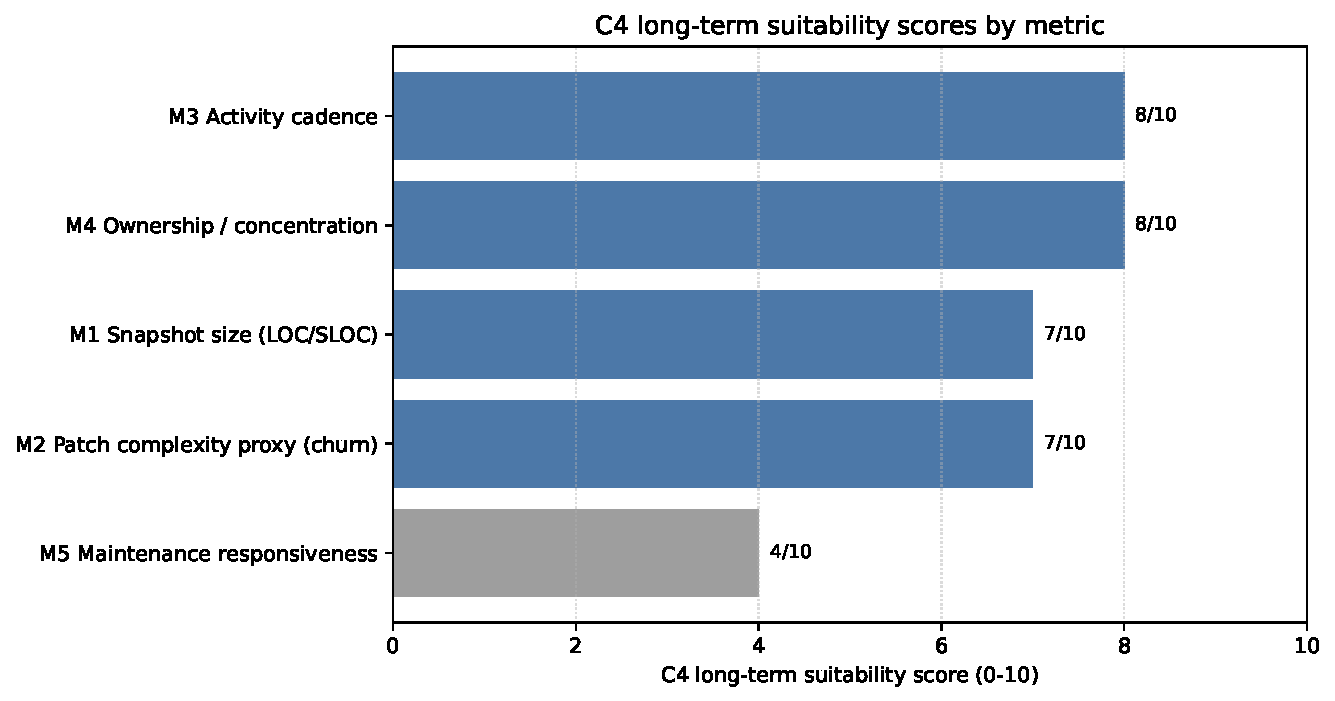
\includegraphics[width=0.90\textwidth]{figures/month3_c4/c4_longterm_suitability_scores.pdf}
\caption{C4 long-term suitability scores on a 0--10 scale. Higher values indicate stronger suitability for long histories.}
\label{fig:c4_longterm_scores}
\end{figure}

C4 does not reverse the earlier findings, but it clarifies their time horizon. M3 is strong for long-term operation
because commit counts, active days, and normalized cadence can be appended window by window and stored compactly.
The limitation is interpretive: activity naturally changes when a project matures, so cadence should not be read
without churn and ownership context. M4 also scores high because relative ownership remains comparable even when
projects differ in size and release rhythm. Its cost is operational rather than conceptual: the system must keep
identity canonicalization and share calculations explicit.

M1 and M2 are useful supporting signals. M1 gives a durable size baseline and denominator, but it does not describe
developer reputation by itself. M2 remains a practical measure of effort over time, but long histories make its
volatility more visible, especially around refactors or formatting-heavy releases. M5 remains outside the baseline
decision because there is no current issue or pull-request event evidence to update, audit, or validate.

\subsection{C4 interpretation for the decision process}
\label{sec:c4_interpretation}

C4 completes the four comparative criteria before smart-contract feasibility scoring:
\begin{itemize}[leftmargin=*]
  \item M3 is operationally attractive because it is compact and incremental, but it needs protection from the C3 gaming risks.
  \item M4 has the strongest long-term reputation fit among implemented metrics, but requires careful identity and state handling.
  \item M1 should remain in the baseline as contextual evidence and normalization support.
  \item M2 should remain available as effort evidence, especially when combined with cadence and ownership checks.
  \item M5 should stay documented for future work and should not enter the current PoC decision.
\end{itemize}

The next step is the smart-contract feasibility scoring pass. That pass should combine the C1--C4 findings with
the predefined feasibility rubric before selecting exactly one metric for the baseline proof-of-concept.
